%%%%%%%%%%%%%%%%%%%%%%%%%%%%%%%%%%%%%%%%%%%%%%%%%%%%%%%%%%%%%%%%%%%%%%%%%%%%%%%%
\chapter{Тестирование прототипа аспектно-ориентированного расширения}
\label{ch:testing}
%%%%%%%%%%%%%%%%%%%%%%%%%%%%%%%%%%%%%%%%%%%%%%%%%%%%%%%%%%%%%%%%%%%%%%%%%%%%%%%%
В данном разделе ставится задача проведения тестирования разработанного прототипа на предмет наличия дефектов и соответствия поставленным функциональным и нефункциональным требованиям.
%%%%%%%%%%%%%%%%%%%%%%%%%%%%%%%%%%%%%%%%%%%%%%%%%%%%%%%%%%%%%%%%%%%%%%%%%%%%%%%%
\section{Программа испытаний}
\label{sec:testing_program}
%%%%%%%%%%%%%%%%%%%%%%%%%%%%%%%%%%%%%%%%%%%%%%%%%%%%%%%%%%%%%%%%%%%%%%%%%%%%%%%%
Для упрощения процесса тестирования, он был разбит на несколько этапов.
Первым этапов является проверка корректности построения срезов, в ходе которого проверяется корректность разбора описания аспектов и построения срезов.
Вторым этапом является проверка корректности внедрения кода совета в PSI целевой программы.
Заключительным этапом является проверка корректности программы после применения к ней аспектов.
%%%%%%%%%%%%%%%%%%%%%%%%%%%%%%%%%%%%%%%%%%%%%%%%%%%%%%%%%%%%%%%%%%%%%%%%%%%%%%%%
\subsection{Проверка правильности построения срезов}
\label{subs:pointcut_testing_program}
Для того, чтобы убедиться в корректности формирования срезов, необходимо проверить:
\begin{itemize}
	\item Поиск узлов программы, соответствующих отдельным сигнатурам.
	\item Формирование срезов при помощи логических операторов.
\end{itemize}
Для этого необходимо убедиться в правильности следующий частей программы:
\begin{enumerate}
    \item \label{list:method_items_check}Проверка корректности разбора описания метода внутри сигнатур описания среза:
    \begin{enumerate}
        \item \label{list:method_name_check}Проверка поиска метода по его имени (в том числе при использовании метасимвола \quotes{*});
        \item \label{list:class_name_check}Проверка поиска метода по имени класса, к которому он принадлежит (в том числе при использовании метасимвола \quotes{*});
        \item \label{list:method_params_check}Проверка поиска метода при указании типов параметров метода с учетом использования nullability модификаторов;
        \item \label{list:method_modifiers_check}Проверка поиска метода по его модификаторам;
        \item \label{list:method_extension_check}Корректность поиска extension методов;
        \item \label{list:method_inline_check}Корректность поиска inline методов;
        \item \label{list:method_return_value_check}Корректность поиска метода по возвращаемому им значению с учетом nullability модификаторов;
    \end{enumerate}
    \item \label{list:pointcut_items_check}Проверка корректности обработка сигнатур описания срезов:
    \begin{enumerate}
        \item \label{list:call_check}Проверка сигнатуры \textit{call};
        \item \label{list:execution_check}Проверка сигнатуры \textit{execution};
        \item \label{list:target_check}Проверка сигнатуры \textit{target} (как в случаях когда внутри сигнатуры описывается только тип, так и когда внутри неё находится идентификатор аргумента совета);
    \end{enumerate}
    \item \label{list:reference_pointcut_check}Проверка корректности использования именованных срезов при описании других срезов;
    \item \label{list:logic_operations_check}Проверка корректности использования операций конъюнкции, дизъюнкции и инверсии.
\end{enumerate}
%%%%%%%%%%%%%%%%%%%%%%%%%%%%%%%%%%%%%%%%%%%%%%%%%%%%%%%%%%%%%%%%%%%%%%%%%%%%%%%%
\subsection{Проверка корректности построения кода совета}
\label{subs:advice_code_testing_program}
%%%%%%%%%%%%%%%%%%%%%%%%%%%%%%%%%%%%%%%%%%%%%%%%%%%%%%%%%%%%%%%%%%%%%%%%%%%%%%%%
После проверки формирования срезов, необходимо убедиться в корректности применения советов, который включает в себя:
\begin{itemize}
	\item Формирование вспомогательного метода, содержащего код совета.
	\item Перенос точки внедрения внутрь враппер-функции.
	\item Вызов вспомогательного метода.
\end{itemize}
Для осуществления проверки применения советов необходимо проверить следующее:
\begin{enumerate}
    \item \label{list:lambda_wrapper_check}Корректность оборачивания точки внедрения в лямбда-враппер;
    \item \label{list:buffer_method_check}Корректность оборачивания кода совета в вспомогательный метод как при использовании сигнатуры \textit{target}, так и без неё;
    \item \label{list:buffer_method_call_check}Корректность передачи значения внутрь вспомогательного метода при использовании сигнатуры \textit{target};
    \item \label{list:pointcut_call_check}Корректность вызова метода, являющегося точкой внедрения, внутри лямбда-враппера;
    \item \label{list:target_use_check}Проверка обращения к элементу, на котором был произведен вызов целевого метода внутри кода совета;
\end{enumerate}
%%%%%%%%%%%%%%%%%%%%%%%%%%%%%%%%%%%%%%%%%%%%%%%%%%%%%%%%%%%%%%%%%%%%%%%%%%%%%%%%
\subsection{Проверка способа внедрения советов}
\label{subs:advice_weaving_testing_program}
%%%%%%%%%%%%%%%%%%%%%%%%%%%%%%%%%%%%%%%%%%%%%%%%%%%%%%%%%%%%%%%%%%%%%%%%%%%%%%%%
После применения кода совета, необходимо убедиться в том, что программа работает согласно нашим ожиданиям:
\begin{itemize}
	\item Не возникает ошибок при компиляции или выполнении программы после применения аспектов.
	\item Код советов работает согласно нашим ожиданиям.
\end{itemize}
Для этого необходимо проверить следующее:
\begin{enumerate}
    \item \label{list:advice_weaving_check}Корректность выполнения кода совета относительно точки внедрения:
    \begin{enumerate}
        \item \label{list:before_advice_weaving_check}При использовании совета \textit{before}, код совета должен быть выполнен до точки внедрения;
        \item \label{list:after_advice_weaving_check}При использовании совета \textit{after}, код совета должен быть выполнен после точки внедрения;
        \item \label{list:around_advice_weaving_check}При использовании совета \textit{around}, код совета должен быть выполнен вместо точки внедрения;
    \end{enumerate}
    \item \label{list:several_advices_weaving_check}Применение нескольких советов к одной точке внедрения;
    \item \label{list:program_work_check}Работу программы после применения аспектов.
\end{enumerate}
%%%%%%%%%%%%%%%%%%%%%%%%%%%%%%%%%%%%%%%%%%%%%%%%%%%%%%%%%%%%%%%%%%%%%%%%%%%%%%%%
\subsection{Проверка работоспособности прототипа на больших проектах}
\label{subs:students_testing_program}
%%%%%%%%%%%%%%%%%%%%%%%%%%%%%%%%%%%%%%%%%%%%%%%%%%%%%%%%%%%%%%%%%%%%%%%%%%%%%%%%
На заключительном этапе, для проверки корректности разработанного прототипа было решено произвести проверку на других проектах.
В качестве целевых программ было решено выбрать студенческие программы.
Данный выбор был произведен по следующим причинам:
\begin{itemize}
	\item Достаточная сложность программ (размер в несколько сотен строк кода, несколько классов);
	\item Достаточная легкость оценки корректности применения аспектов к программе.
\end{itemize}
%%%%%%%%%%%%%%%%%%%%%%%%%%%%%%%%%%%%%%%%%%%%%%%%%%%%%%%%%%%%%%%%%%%%%%%%%%%%%%%%
\section{Методика испытаний}
\label{sec:testing_methodology}
%%%%%%%%%%%%%%%%%%%%%%%%%%%%%%%%%%%%%%%%%%%%%%%%%%%%%%%%%%%%%%%%%%%%%%%%%%%%%%%%
Для проведения функционального тестирования было решено составить целевую программу, состоящую из трех файлов: \textit{Main.kt} (приложение \ref{listings:target_Main.kt}), \textit{Foo.kt} (приложение~\ref{listings:target_Foo}) и \textit{Bar.kt} (приложение~\ref{listings:target_Bar.kt}).
Файл \textit{Main.kt} является точкой входа в программу и содержит метод \textit{main}.
Файлы \textit{Foo.kt} и \textit{Bar.kt} содержат классы \textit{Foo} и \textit{Bar} соответственно.
Также данные классы содержат различные целевые методы, как, например, inline и execution методы, методы с различными аргументами, модификаторами и т.д.
%%%%%%%%%%%%%%%%%%%%%%%%%%%%%%%%%%%%%%%%%%%%%%%%%%%%%%%%%%%%%%%%%%%%%%%%%%%%%%%%
\subsection{Методика проверки корректности формирования срезов}
\label{sub:pointcut_building_methodology}
%%%%%%%%%%%%%%%%%%%%%%%%%%%%%%%%%%%%%%%%%%%%%%%%%%%%%%%%%%%%%%%%%%%%%%%%%%%%%%%%
Для проверки корректности пунктов
\quotes{\ref{list:method_name_check}},
\quotes{\ref{list:class_name_check}},
\quotes{\ref{list:method_params_check}},
\quotes{\ref{list:call_check}},
\quotes{\ref{list:reference_pointcut_check}} подраздела~\ref{subs:pointcut_testing_program} используется аспект, приведенный в листинге~\ref{lst:test_aspect_1}:
\begin{lstlisting}[style={java}, label={lst:test_aspect_1},
  caption={Пример тестового аспекта}]
aspect A  {
    pointcut FooPC(): call(fun foo())

    before(): FooPC() {
        println("foo")
    }
}
\end{lstlisting}
% Как видно из листинга~\ref{lst:test_aspect_1}, представленный аспект содержит в себе одно описание среза и один совет \textit{before}.
% Данный совет должен быть применен перед всеми точками внедрения, принадлежащих срезу \textit{FooPC}.
% Исходя из описания среза, в него попадают места, в которых происходит вызов метода \textit{foo}, не принимающего аргументов и не возвращающего никакого значения.

% Исходя из архитектуры целевой программы, в срез должен попасть только вызов метода \textit{foo()} внутри метода \textit{main}.
Ожидается, что в результирующий срез попадут только места программы, в которых производится вызов метода \textit{foo()}.

 Для проверки корректности пунктов
 \quotes{\ref{list:method_name_check}},
 \quotes{\ref{list:class_name_check}},
 \quotes{\ref{list:method_modifiers_check}},
 \quotes{\ref{list:method_return_value_check}},
 \quotes{\ref{list:execution_check}},
 \quotes{\ref{list:reference_pointcut_check}},
 \quotes{\ref{list:logic_operations_check}} подраздела~\ref{subs:pointcut_testing_program} используется аспект, приведенный в листинге~\ref{lst:test_aspect_2}:
\begin{lstlisting}[style={java}, label={lst:test_aspect_2},
  caption={Пример тестового аспекта}]
aspect B  {
    pointcut BarPC(): call(!private fun b*(Int, Foo?): Boolean)

    after(): BarPC() && execution(fun Foo.foo()){
        println("b* call")
    }
}
\end{lstlisting}
% Как видно из листинга~\ref{lst:test_aspect_2}, представленный аспект содержит в себе одно описание среза и один совет \textit{after}.
% Данный совет должен быть применен перед всеми точками внедрения, принадлежащих срезу \textit{BarPC} которые находятся внутри тела метода \textit{foo()}, принадлежащего классу \textit{Foo}.
% Исходя из описания среза, в него попадают места, в которых происходит вызов метода, начинающегося с символа \quotes{b}.
% Также данный метод должен принимать два аргумента:
% \begin{enumerate}
% 	\item аргумент типа \textit{Int}, который может быть как \textit{Nullable}, так и \textit{NotNull};
% 	\item аргумент типа \textit{Foo}, который может принимать значение \textit{Null}.
% \end{enumerate}
% и возвращать значение типа \textit{Boolean}, которые не должно принимать значение \textit{null}.

% Исходя из архитектуры целевой программы, в срез должен попасть только вызов метода \textit{bar(a: Int, b: Foo?): Boolean} внутри метода \textit{foo()}.
Ожидается, что в итоговый срез попадут только места в программе, которые принадлежат срезу \textit{BarPC} и соответствуют описанию внутри сигнатуры \textit{execution}.

Для проверки корректности пунктов \quotes{\ref{list:method_name_check}},
\quotes{\ref{list:class_name_check}},
\quotes{\ref{list:method_params_check}},
\quotes{\ref{list:method_modifiers_check}},
\quotes{\ref{list:method_extension_check}},
\quotes{\ref{list:method_return_value_check}},
\quotes{\ref{list:target_check}},
\quotes{\ref{list:logic_operations_check}} подраздела~\ref{subs:pointcut_testing_program} используется аспект, приведенный в листинге~\ref{lst:test_aspect_3}:
\begin{lstlisting}[style={java}, label={lst:test_aspect_3},
  caption={Пример тестового аспекта}]
aspect C  {
    around(): target(Foo) && call(extension fun Foo.b*z(String!!): Boolean!!){
        println("b* call")
    }
}
\end{lstlisting}
% Как видно из листинга~\ref{lst:test_aspect_2}, представленный аспект содержит в себе один совет \textit{around}.
% Данный совет должен быть применен вместо всех методов которые вызываются на элементе типа \textit{Foo}.
% Также имя этих методов должно начинаться с символа \quotes{b} и заканчиваться символом \textit{z}, принимать единственный аргумент типа \textit{String}, который не может принимать значение \textit{null} и возвращать значение типа \textit{Boolean}, которое также не может принимать значение \textit{null}.
% Также метод, попадающий в срез, к котором будет применен совет должен быть extension методом.

% Исходя из архитектуры целевой программы, в срез должен попасть только вызов метода \textit{Foo.baz(s: String): Boolean} внутри метода \textit{main}.
Ожидается, что в срез попадут только места в программе, которые соответствуют сигнатуре \textit{call}, при этом их вызов должен производиться на элементе типа \textit{Foo}.

Совет, представленный в листинге~\ref{lst:test_aspect_4} аналогичен совету из листинга~\ref{lst:test_aspect_3}, однако в данном примере тип, на котором должен производиться вызов целевого метода не задан явно внутри сигнатуры \textit{target}.
Данный формат записи сигнатуры \textit{target} позволяет обращаться к элементу, на котором был произведен вызов метода, внутри кода совета.
Вместо этого в данной сигнатуре указывается идентификатор аргумента совета и при формировании среза тип берется из списка параметров метода.
\begin{lstlisting}[style={java}, label={lst:test_aspect_4},
  caption={Пример тестового аспекта}]
aspect D {
    around(foo: Foo): target(foo) && call(extension fun Foo.b*z(String!!): Boolean!!){
        println("b* call")
    }
}
\end{lstlisting}
Так как точки программы, попадающие в описание среза представленного в листинге~\ref{lst:test_aspect_4} эквивалентны точкам, попадающим в срез, описанный в листинге~\ref{lst:test_aspect_3}, в срез должен попасть только вызов метода \textit{Foo.baz(s: String): Boolean} внутри метода \textit{main}.

Для проверки корректности пунктов \quotes{\ref{list:method_name_check}},
\quotes{\ref{list:class_name_check}},
\quotes{\ref{list:method_params_check}},
\quotes{\ref{list:method_modifiers_check}},
\quotes{\ref{list:method_inline_check}},
\quotes{\ref{list:logic_operations_check}} подраздела~\ref{subs:pointcut_testing_program} используется аспект, приведенный в листинге~\ref{lst:test_aspect_5}:
\begin{lstlisting}[style={java}, label={lst:test_aspect_5},
  caption={Пример тестового аспекта}]
aspect E {
    before(): call(!inline fun Foo.*(String)){
        println("hello non inline from advice")
    }
}
\end{lstlisting}
% Как видно из листинга~\ref{lst:test_aspect_5}, представленный аспект содержит в себе один совет \textit{before}.
% В срез, описанный в данном совете, попадают все места вызовов методов в программе, при этом метод должен удовлетворять следующим требованиям:
% \begin{enumerate}
% 	\item должен принадлежать классу \textit{Foo};
% 	\item должен принимать единственный аргумент типа \textit{String};
% 	\item не должен быть \textit{inline} методом.
% \end{enumerate}
% Исходя из архитектуры программы, в срез, описанный в совете, должен попасть только вызов метода \textit{nonInlineFas(str: String)}.
Ожидается, что в описанный срез попадут не \textit{inline} методы класса \textit{Foo}, принимающие единственный аргумент типа \textit{String} и возвращающие значения типа \textit{Boolean}.

 Для проверки корректности пунктов
 \quotes{\ref{list:method_name_check}},
 \quotes{\ref{list:class_name_check}},
 \quotes{\ref{list:logic_operations_check}} подраздела~\ref{subs:pointcut_testing_program} используется аспект, приведенный в листинге~\ref{lst:test_aspect_6}:
\begin{lstlisting}[style={java}, label={lst:test_aspect_6},
  caption={Пример тестового аспекта}]
aspect B  {
    before(): call(fun bas(String): Boolean) || call(fun baz(String): Boolean){
        println("or call")
    }
}
\end{lstlisting}
При применении данного аспекта проверяется не только корректность использования сигнатур при описании среза, но и использовании операции дизъюнкции при описании срезов.
Ожидаемым результатом является то, что в срез попадут места в программе, соответствующие как минимум одной из сигнатур, содержащихся в описании среза.
%%%%%%%%%%%%%%%%%%%%%%%%%%%%%%%%%%%%%%%%%%%%%%%%%%%%%%%%%%%%%%%%%%%%%%%%%%%%%%%%
\subsection{Методика проверки корректности построения кода совета}
\label{sub:advice_building_methodology}
%%%%%%%%%%%%%%%%%%%%%%%%%%%%%%%%%%%%%%%%%%%%%%%%%%%%%%%%%%%%%%%%%%%%%%%%%%%%%%%%
Для проверки корректности пунктов \quotes{\ref{list:lambda_wrapper_check}},
\quotes{\ref{list:buffer_method_check}},
\quotes{\ref{list:pointcut_call_check}} подраздела \ref{subs:advice_weaving_testing_program}  используется аспект, приведенный в листинге~\ref{lst:test_aspect_2_1}:
\begin{lstlisting}[style={java}, label={lst:test_aspect_2_1},
  caption={Пример тестового аспекта}]
aspect B  {
    pointcut BarPC(): call(!private fun b*(Int, Foo?): Boolean)

    after(): BarPC() && execution(fun Foo.foo()){
        println("b* call")
    }
}
\end{lstlisting}
% Так как рассматриваемый аспект не содержит в описании среза сигнатуру \textit{target}, точка внедрения должна быть обернута в лямбда-враппер \textit{run}.
% Код совета должен быть вынесен в отдельный вспомогательный метод, не принимающий параметров и не возвращающий никакого значения.
% При вызове метода внутри лямбда-враппера, в него не должны передаваться никакие аргументы и возвращаемое им значение не должно присваиваться никакой переменной.
% При вызове метода, являющегося точкой внедрения, необходимо передавать туда те аргументы, которые передавались и при вызове метода до применения аспекта.
Ожидаемым результатом применения аспекта является оборачивание точки внедрения в лябда-враппер \textit{run}.
Вспомогательный метод, содержащий код совета, не должен принимать никаких аргументов.

Для проверки корректности пунктов \quotes{\ref{list:lambda_wrapper_check}},
\quotes{\ref{list:buffer_method_check}},
\quotes{\ref{list:buffer_method_call_check}},
\quotes{\ref{list:pointcut_call_check}},
\quotes{\ref{list:target_use_check}}, подраздела \ref{subs:advice_weaving_testing_program}  используется аспект, приведенный в листинге~\ref{lst:test_aspect_2_2}:
\begin{lstlisting}[style={java}, label={lst:test_aspect_2_2},
  caption={Пример тестового аспекта}]
aspect D {
    before(foo: Foo): target(foo) && call(extension fun Foo.b*z(String!!): Boolean!!){
        foo.foo()
    }
}
\end{lstlisting}
% Так как рассматриваемый аспект содержит в описании среза сигнатуру \textit{target}, принимающую в качестве аргумента параметр совета, точка внедрения должна быть обернута в лямбда-враппер \textit{let}.
% Внутри \textit{let} должен быть явно указан аргумент метода.
% Код совета должен быть вынесен в отдельный вспомогательный метод, принимающий в качестве первого аргумента элемент типа, используемого в сигнатуре \textit{target} и не возвращающий никакого значения.
% При вызове метода внутри лямбда-враппера, в него в качестве первого аргумента должен передаваться аргумент лямбда-враппера, а возвращаемое им значение не должно присваиваться никакой переменной.
% При вызове метода, являющегося точкой внедрения, необходимо передавать туда те аргументы, которые передавались и при вызове метода до применения аспекта.
% Вызов метода должен осуществляться на аргументе враппера \textit{let}.
Ожидаемым результатом применения этого аспекта является помещение точки внедрения внутрь лямбда-враппера \textit{let}.
Аргумент метода \textit{let} должен передаваться в качестве первого аргумента при вызове метода, содержащего код совета.
Вызов метода, являющегося точкой внедрения, должен осуществляться на аргументе враппера \textit{let}.
%%%%%%%%%%%%%%%%%%%%%%%%%%%%%%%%%%%%%%%%%%%%%%%%%%%%%%%%%%%%%%%%%%%%%%%%%%%%%%%%
\subsection{Методика проверки корректности внедрения кода совета}
\label{sub:advice_weaving_methodology}
%%%%%%%%%%%%%%%%%%%%%%%%%%%%%%%%%%%%%%%%%%%%%%%%%%%%%%%%%%%%%%%%%%%%%%%%%%%%%%%%
Для проверки корректности пунктов \quotes{\ref{list:before_advice_weaving_check}},
\quotes{\ref{list:program_work_check}}  подраздела \ref{subs:advice_weaving_testing_program} используется аспект, приведенный в листинге \ref{lst:test_aspect_3_1}:
\begin{lstlisting}[style={java}, label={lst:test_aspect_3_1},
  caption={Пример тестового аспекта}]
aspect A  {
    before(): call(fun foo()) {
        println("before test mes")
    }
}
\end{lstlisting}
% Описанный в листинге \ref{lst:test_aspect_3_1} совет должен быть применен перед всеми местами в программе, в которых происходит вызов метода \textit{foo()}.
% Ожидается, что при применении данного совета, вспомогательный метод, содержащий код совета, будет выполнен раньше, чем точка внедрения.
Ожидаемым результатом применения аспекта является  вывод на консоль отладочного сообщения \quotes{before test mes} перед отладочными сообщениями, выводимыми внутри метода \textit{foo()}.

Для проверки корректности пунктов \quotes{\ref{list:after_advice_weaving_check}},
\quotes{\ref{list:program_work_check}}  подраздела \ref{subs:advice_weaving_testing_program} используется аспект, приведенный в листинге \ref{lst:test_aspect_3_2}:
\begin{lstlisting}[style={java}, label={lst:test_aspect_3_2},
  caption={Пример тестового аспекта}]
aspect A  {
    after(): call(fun foo()) {
        println("after test mes")
    }
}
\end{lstlisting}
% Описанный в листинге \ref{lst:test_aspect_3_2} совет должен быть применен после всеми местами в программе, в которых происходит вызов метода \textit{foo()}.
% Ожидается, что при применении данного совета, вспомогательный метод, содержащий код совета, будет выполнен позже, чем точка внедрения.
Ожидаемым результатом применения аспекта является вывод на консоль отладочного сообщения \quotes{after test mes} после отладочных сообщений, выводимыми внутри метода \textit{foo()}.

Для проверки корректности пунктов \quotes{\ref{list:around_advice_weaving_check}},
\quotes{\ref{list:program_work_check}}  подраздела \ref{subs:advice_weaving_testing_program} используется аспект, приведенный в листинге \ref{lst:test_aspect_3_3}:
\begin{lstlisting}[style={java}, label={lst:test_aspect_3_3},
  caption={Пример тестового аспекта}]
aspect A  {
    around(foo: Foo): call(fun foo()) && target(foo){
        foo.nonInlineFas("Around message")
    }
}
\end{lstlisting}
% Описанный в листинге \ref{lst:test_aspect_3_3} совет должен быть применен вместо всеи местами в программе, в которых происходит вызов метода \textit{foo()}.
% Ожидается, что при применении данного совета, вспомогательный метод, содержащий код совета, будет выполнен вместо точки внедрения.
Ожидаемым результатом применения аспекта является вывод на консоль отладочного сообщения \quotes{around test mes} вместо отладочных сообщений, выводимых внутри метода \textit{foo()}.

Для проверки корректности пунктов \quotes{\ref{list:before_advice_weaving_check}},
\quotes{\ref{list:after_advice_weaving_check}},
\quotes{\ref{list:several_advices_weaving_check}},
\quotes{\ref{list:program_work_check}}  подраздела \ref{subs:advice_weaving_testing_program} используется аспект, приведенный в листинге \ref{lst:test_aspect_3_4}:
\begin{lstlisting}[style={java}, label={lst:test_aspect_3_4},
  caption={Пример тестового аспекта}]
aspect A  {
    pointcut FooPC(): call(fun foo())

    before(): FooPC() {
        println("before message")
    }

    after(): FooPC() {
        println("after message")
    }

}
\end{lstlisting}
Ожидаемым результатом применения аспекта будет вывод на консоль отладочного сообщения \quotes{before message} до сообщений, выводимых внутри метода \textit{foo()}, и вывод сообщения \textit{after message} после.
%%%%%%%%%%%%%%%%%%%%%%%%%%%%%%%%%%%%%%%%%%%%%%%%%%%%%%%%%%%%%%%%%%%%%%%%%%%%%%%%
\subsection{Методика проверки корректности прототипа на больших проектах}
\label{sub:students_programm_methodology}
%%%%%%%%%%%%%%%%%%%%%%%%%%%%%%%%%%%%%%%%%%%%%%%%%%%%%%%%%%%%%%%%%%%%%%%%%%%%%%%%
Для проверки согласно методике, описанной в подразделе~\ref{subs:students_testing_program} используется аспект, приведенный в листинге \ref{lst:test_aspect_4_1}:
\begin{lstlisting}[style={java}, label={lst:test_aspect_4_1},
  caption={Пример тестового аспекта}]
aspect A  {
  pointcut pExprPC() : execution(fun parseExpr(String, List<Int>): Map<Int, Int> )
  pointcut calcPC() : call(fun Expression.calculate(Int): Int)

  before(): pExprPC() && calcPC() {
    val l = java.util.logging.Logger.getLogger("ALog")
    l.info("Start ${System.currentTimeMillis()}")
  }

  after(): pExprPC() && calcPC() {
    val l = java.util.logging.Logger.getLogger("ALog")
    l.info("Finish ${System.currentTimeMillis()}")
  }
}
\end{lstlisting}
Ожидаемым результатом применения аспекта будет вывод в лог времени вызова метода \textit{calculate} и времени окончания его работы.
При этом, должно протоколироваться только вызов метода, находящийся внутри тела метода \textit{parseExpr}, так как данный вызов является точкой входа в вычисление значения выражения.
%%%%%%%%%%%%%%%%%%%%%%%%%%%%%%%%%%%%%%%%%%%%%%%%%%%%%%%%%%%%%%%%%%%%%%%%%%%%%%%%

% В листинге \ref{lst:test_aspect_3_4} описан срез \textit{FooPC}, включающий в себя все места в программе, в которых происходит вызов метода \textit{foo()}.
% Также внутри аспекта представлено два совета: \textit{before} и \textit{after}, которые должны быть применены до и после точек внедрения, попадающий в срез \textit{FooPC}, соответственно.
% Ожидается, что к точке внедрения будет сначала применен один из советов, потом другой.
% При этом, каждый из советов должен выполняться корректно.
% Порядок применения советов к точке внедрения не регламентирован.
% Следствием этого будет вывод на консоль отладочного сообщения \quotes{before message} до отладочных сообщений, выводимых внутри метода \textit{foo()}, и сообщение \textit{after message} после.

% Для проведения тестирования был составлен набор аспектов.
% Тестовый набор аспектов должен иметь следующие характеристики:
% \begin{itemize}
% 	\item Набор аспектов должен включать в себя реализованные способы описания срезов: call, execution, target;
% 	\item Набор аспектов должен включать в себя реализованные способы внедрения советов: after, before, around;
% 	\item Описание срезов должно включать в себя обращение к другим срезам;
% 	\item В одном из советов должно производиться обращение к элементам, на которых был произведен вызов метода, попадающего в срез;
% \end{itemize}

% Первым этапом является проверка корректности грамматики, основной целью которого является проверка корректности разбора описания совета и построения дерева разбора.
% Для этой цели было решено воспользоваться средствами плагина для среды разработки IntelliJ IDEA~\cite{antlr_plugin}, который позволяет визуализировать дерево разбора, что является очень удобный для анализа.

% Следующим этапом является функциональное тестирование проекта.
% Как было сказано ранее, из-за сложности проверки PSI в функциональных тестах, при функциональном тестировании было решено сосредоточиться на корректности разбора аспектов и на правильности составления модели аспектов.
% Функциональное тестирование было решено производить при помощи Unit-тестов, используя фреймворк JUnit~4.
% Для проведения функционального тестирования был разработан набор аспектов, по которым происходит построение модели аспекта и сравнение полученной модели с ожидаемым результатом.

% Третьим этапом является проведение функционального тестирования, основная задача которого нахождение ошибок, связанных с построением срезов и применением кода совета к точке внедрения.
% Также на данном этапе проверяется корректность и работоспособность целевой программы после применения советов.

% Для проведения функционального тестирования было решено составить целевую программу, состоящую из трех файлов: \textit{Main.kt} (приложение \ref{listings:target_Main.kt}), \textit{Foo.kt} (приложение~\ref{listings:target_Foo.kt}) и \textit{Bar.kt} (приложение~\ref{listings:target_Bar.kt}).
% Файл \textit{Main.kt} является точкой входа в программу и содержит метод \textit{main}.
% Файлы \textit{Foo.kt} и \textit{Bar.kt} содержат классы \textit{Foo} и \textit{Bar} соответственно.
% Также данные классы содержат различные целевые методы, как, например, inline и execution методы, методы с различными аргументами, модификаторами и т.д.

% Для проверки корректности выделения срезов было решено организовать эксперимент следующим образом:
% \begin{itemize}
%  	\item Составить набор аспектов таким образом, чтобы с одной стороны они включали в себя все реализованные возможности и с другой --- были очевидны места в программе, к которым они будут применены.
%  	\item Задать генерируемым переменным и методам фиксированные имена.
%  	\item Сформировать набор эталонных файлов, представляющих из себя исходные файлы целевой программы, к которой вручную были применены аспекты.
%  	\item После модификации PSI, преобразовать модифицированный PSI в текст программы.
%  	\item Сравнить на равенство полученный текст программы с эталонным на уровне токенов, предварительно, убрав символы форматирования из обоих файлов.
%  \end{itemize}

%  Заключительным этапом проверки качества разработанного прототипа является проверка корректности работы программы после применения аспектов.
%  Самым простым способом данной проверки является вывод отладочных сообщений во время работы программы.
%  На первых этапах было решено проверять корректность работы после применения аспектов на целевой программе, а после --- на более больших проектах (размером несколько сотен строк кода и более).
%%%%%%%%%%%%%%%%%%%%%%%%%%%%%%%%%%%%%%%%%%%%%%%%%%%%%%%%%%%%%%%%%%%%%%%%%%%%%%%%
\section{Проведение испытаний}
\label{sec:testing_run}
%%%%%%%%%%%%%%%%%%%%%%%%%%%%%%%%%%%%%%%%%%%%%%%%%%%%%%%%%%%%%%%%%%%%%%%%%%%%%%%%
Для проверки корректности системы необходимо провести серию экспериментов в соответствии с методикой тестирования, описанной в разделе~\ref{sec:testing_methodology}.
%%%%%%%%%%%%%%%%%%%%%%%%%%%%%%%%%%%%%%%%%%%%%%%%%%%%%%%%%%%%%%%%%%%%%%%%%%%%%%%%
\subsection{Проверка корректности построения срезов}
\label{sub:pointcut_building_tests}
%%%%%%%%%%%%%%%%%%%%%%%%%%%%%%%%%%%%%%%%%%%%%%%%%%%%%%%%%%%%%%%%%%%%%%%%%%%%%%%%
Для проверки корректности пунктов
\quotes{\ref{list:method_name_check}},
\quotes{\ref{list:class_name_check}},
\quotes{\ref{list:method_params_check}},
\quotes{\ref{list:call_check}},
\quotes{\ref{list:reference_pointcut_check}} подраздела~\ref{subs:pointcut_testing_program} воспользуемся аспектом, приведенным в листинге~\ref{lst:test_aspect_1}.
После применения аспекта, текст программы был изменен следующим образом:
\begin{lstlisting}[style={java}, label={lst:result_of_weaving_1_1},
 caption={Результат применения аспекта, описанного в листинге~\ref{lst:test_aspect_1}, к тестовой программе}]
...
f.run{
	fun adviceFun(){
		println ( "foo" )
	}
	adviceFun()
	foo()
}
...
\end{lstlisting}
Из данного преобразования можно сделать вывод о том, что в срез попал только вызов метода \textit{foo()}, что соответствует ожиданиям.

Для проверки корректности пунктов
 \quotes{\ref{list:method_name_check}},
 \quotes{\ref{list:class_name_check}},
 \quotes{\ref{list:method_modifiers_check}},
 \quotes{\ref{list:method_return_value_check}},
 \quotes{\ref{list:execution_check}},
 \quotes{\ref{list:reference_pointcut_check}},
 \quotes{\ref{list:logic_operations_check}} подраздела~\ref{subs:pointcut_testing_program} воспользуемся аспектом, приведенным в листинге~\ref{lst:test_aspect_2}.
 \begin{lstlisting}[style={java}, label={lst:result_of_weaving_1_2},
 caption={Результат применения аспекта, описанного в листинге~\ref{lst:test_aspect_2}, к тестовой программе}]
...
run{
	fun adviceFun(){
        println("b* call")
    }
	val ____a = bar(1,this)
	adviceFun()
	____a
}
...
\end{lstlisting}
Из данного преобразования можно сделать вывод о том, что в срез попал только вызов метода \textit{bar}, находящийся внутри тела метода \textit{foo}, что соответствует ожиданиям.
Вызов метода \textit{bar} внутри метода \textit{main} не попал в срез совета, так как это противоречит сигнатуре \textit{execution(fun Foo.foo())}.

Для проверки корректности пунктов \quotes{\ref{list:method_name_check}},
\quotes{\ref{list:class_name_check}},
\quotes{\ref{list:method_params_check}},
\quotes{\ref{list:method_modifiers_check}},
\quotes{\ref{list:method_extension_check}},
\quotes{\ref{list:method_return_value_check}},
\quotes{\ref{list:target_check}},
\quotes{\ref{list:logic_operations_check}} подраздела~\ref{subs:pointcut_testing_program} воспользуемся аспектом, приведенным в листинге~\ref{lst:test_aspect_3}.
\begin{lstlisting}[style={java}, label={lst:result_of_weaving_1_3},
 caption={Результат применения аспекта, описанного в листинге~\ref{lst:test_aspect_3}, к тестовой программе}]
...
f.run{
	fun adviceFun(){
        println("b* call")
    }
	adviceFun()
}
...
\end{lstlisting}
Преобразование, представленное в листинге~\ref{lst:result_of_weaving_1_3}, было выполнено в том участке программы, где производился вызов метода \textit{baz} на элементе, имеющий тип \textit{Foo}, из чего можно сделать вывод, что срез был построен корректно.

При применении к программе аспекта, описанного в листинге~\ref{lst:test_aspect_4}, совет применяется к тем же местам в программе, что и в предыдущем эксперименте.
Из этого можно сделать вывод о том, что при использовании в сигнатуре \textit{taget} идентификатора параметра совета, построение срезов работает корректно.

Для проверки корректности пунктов \quotes{\ref{list:method_name_check}},
\quotes{\ref{list:class_name_check}},
\quotes{\ref{list:method_params_check}},
\quotes{\ref{list:method_modifiers_check}},
\quotes{\ref{list:method_inline_check}},
\quotes{\ref{list:logic_operations_check}} подраздела~\ref{subs:pointcut_testing_program} воспользуемся аспектом, приведенным в листинге~\ref{lst:test_aspect_5}.
\begin{lstlisting}[style={java}, label={lst:result_of_weaving_1_5},
 caption={Результат применения аспекта, описанного в листинге~\ref{lst:test_aspect_5}, к тестовой программе}]
...
this.run{
	fun adviceFun(){
        println("hello non inline from advice")
    }
	adviceFun()
	nonInlineFas("Hello from non inline")
}
...
\end{lstlisting}
Как видно из листинга~\ref{lst:result_of_weaving_1_5}, совет был применен к месту вызова метода \textit{nonInlineFas}, что соответствует ожиданиям.

 Для проверки корректности пунктов
 \quotes{\ref{list:method_name_check}},
 \quotes{\ref{list:class_name_check}},
 \quotes{\ref{list:logic_operations_check}} подраздела~\ref{subs:pointcut_testing_program} воспользуемся аспектом, приведенным в листинге~\ref{lst:test_aspect_6}.
 \begin{lstlisting}[style={java}, label={lst:result_of_weaving_1_6},
 caption={Результат применения аспекта, описанного в листинге~\ref{lst:test_aspect_6}, к тестовой программе}]
...
f.run{
	fun adviceFun1(){
        println("or call")
    }
	adviceFun1()
	baz("PSS")
}

f.run{
	fun adviceFun2(){
        println("or call")
    }
	adviceFun2()
	bas("SPP")
}
...
\end{lstlisting}
Как видно из листинга~\ref{lst:result_of_weaving_1_6}, в срез, к которым был применен совет, попали как вызов метода \textit{baz}, так и вызов метода \textit{bas}, из чего можно сделать вывод о том, что срез строится корректно при использовании операции дизъюнкции.
%%%%%%%%%%%%%%%%%%%%%%%%%%%%%%%%%%%%%%%%%%%%%%%%%%%%%%%%%%%%%%%%%%%%%%%%%%%%%%%%
\subsection{Проверка корректности построения кода совета}
\label{sub:advice_code_building_tests}
%%%%%%%%%%%%%%%%%%%%%%%%%%%%%%%%%%%%%%%%%%%%%%%%%%%%%%%%%%%%%%%%%%%%%%%%%%%%%%%%
Для проверки корректности пунктов \quotes{\ref{list:lambda_wrapper_check}},
\quotes{\ref{list:buffer_method_check}},
\quotes{\ref{list:pointcut_call_check}} подраздела \ref{subs:advice_weaving_testing_program} воспользуемся аспектом, приведенным в листинге~\ref{lst:test_aspect_2_1}.
\begin{lstlisting}[style={java}, label={lst:result_of_weaving_2_1},
 caption={Результат применения аспекта, описанного в листинге~\ref{lst:test_aspect_2_1}, к тестовой программе}]
...
run{
	fun adviceFun(){
        println("b* call")
    }
	val ____a = bar(1,this)
	adviceFun()
	____a
}
...
\end{lstlisting}
Как видно из результатов преобразования, представленных в листинге~\ref{lst:result_of_weaving_2_1}, точка внедрения была обернута в лямбда-враппер \textit{run}.
Код совета был обернут в вспомогательный метод, не принимающий аргументов и не возвращающий значения.
Данный метод был вызван после точки внедрения, а результат, возвращенный точкой внедрения был сохранен в промежуточную переменную и возвращен из враппера.
Исходя из описанного выше, можно сделать вывод о том, что совет был корректно применен к точке внедрения.

Для проверки корректности пунктов \\quotes{\ref{list:lambda_wrapper_check}},
\quotes{\ref{list:buffer_method_check}},
\quotes{\ref{list:buffer_method_call_check}},
\quotes{\ref{list:pointcut_call_check}},
\quotes{\ref{list:target_use_check}} подраздела \ref{subs:advice_weaving_testing_program} воспользуемся аспектом, приведенным в листинге~\ref{lst:test_aspect_2_2}.
\begin{lstlisting}[style={java}, label={lst:result_of_weaving_2_2},
 caption={Результат применения аспекта, описанного в листинге~\ref{lst:test_aspect_2_2}, к тестовой программе}]
...
f.let{ adviceIt ->
	fun adviceFun(foo: Foo){
    	foo.foo()
    }
	adviceFun(adviceIt)
	adviceIt.baz("PSS")
}
...
\end{lstlisting}
Как видно из результатов преобразования, представленных в листинге~\ref{lst:result_of_weaving_2_2}, точка внедрения была обернута в лямбда-враппер \textit{let} с параметром \textit{adviceIt}.
Код совета был обернут в вспомогательный метод, принимающий аргумент \textit{foo: Foo} и не возвращающий значения.
Данный метод был вызван до точки внедрения, а точка внедрения была вызвана на параметре обертке \textit{adviceIt}.
Исходя из описанного выше, можно сделать вывод о том, что совет был корректно применен к точке внедрения.
%%%%%%%%%%%%%%%%%%%%%%%%%%%%%%%%%%%%%%%%%%%%%%%%%%%%%%%%%%%%%%%%%%%%%%%%%%%%%%%%
\subsection{Проверка корректности внедрения советов}
\label{sub:advice_code_weaving_tests}
%%%%%%%%%%%%%%%%%%%%%%%%%%%%%%%%%%%%%%%%%%%%%%%%%%%%%%%%%%%%%%%%%%%%%%%%%%%%%%%%
Для проверки корректности пунктов \quotes{\ref{list:before_advice_weaving_check}},
\quotes{\ref{list:program_work_check}}  подраздела \ref{subs:advice_weaving_testing_program} воспользуемся аспектом, приведенным в листинге \ref{lst:test_aspect_3_1}.
\begin{lstlisting}[style={java}, label={lst:result_of_weaving_3_1},
 caption={Результат применения аспекта, описанного в листинге~\ref{lst:test_aspect_3_1}, к тестовой программе}]
...
f.run{
	fun adviceFun(){
		println ( "foo" )
	}
	adviceFun()
	foo()
}
...
\end{lstlisting}
Как видно из листинга, метод, содержащий код совета, вызывается до точки внедрения.
В листинге~\ref{lst:output_after_weaving_3_1} представлен результат работы программы после применения аспекта, описанного в листинге~\ref{lst:test_aspect_3_1}. 
\begin{lstlisting}[style={java}, label={lst:output_after_weaving_3_1},
 caption={Результат работы программы после применения аспекта, описанного в листинге~\ref{lst:test_aspect_3_1}}]
before test mes
Hello world
Bar hello
Say hello again
Hello from inline
Hello from non inline
Bar hello
PSS Baz!!
SPP Baz!!
Hello from Bar.bar
\end{lstlisting}
Как видно из листинга~\ref{lst:test_aspect_3_1}, тестовое сообщение, выводимое в коде совета, было выведено до начала работы метода \textit{foo()}, что свидетельствует о корректности применения совета.

Для проверки корректности пунктов \quotes{\ref{list:after_advice_weaving_check}},
\quotes{\ref{list:program_work_check}}  подраздела \ref{subs:advice_weaving_testing_program} воспользуемся аспектом, приведенным в листинге \ref{lst:test_aspect_3_2}.
\begin{lstlisting}[style={java}, label={lst:result_of_weaving_3_2},
 caption={Результат применения аспекта, описанного в листинге~\ref{lst:test_aspect_3_2}, к тестовой программе}]
...
f.run{
	fun adviceFun(){
        println("after test mes")
    }
	val ____a = foo()
	adviceFun()
	____a
}
...
\end{lstlisting}
Как видно из листинга, метод, содержащий код совета, вызывается после точки внедрения.
В листинге~\ref{lst:output_after_weaving_3_2} представлен результат работы программы после применения аспекта, описанного в листинге~\ref{lst:test_aspect_3_2}. 
\begin{lstlisting}[style={java}, label={lst:output_after_weaving_3_2},
 caption={Результат работы программы после применения аспекта, описанного в листинге~\ref{lst:test_aspect_3_2}}]
Hello world
Bar hello
Say hello again
Hello from inline
Hello from non inline
after test mes
Bar hello
PSS Baz!!
SPP Baz!!
Hello from Bar.bar
\end{lstlisting}
Как видно из листинга~\ref{lst:test_aspect_3_2}, тестовое сообщение, выводимое в коде совета, было выведено после окончания работы метода \textit{foo()}, что свидетельствует о корректности применения совета.

Для проверки корректности пунктов \quotes{\ref{list:around_advice_weaving_check}},
\quotes{\ref{list:program_work_check}}  подраздела \ref{subs:advice_weaving_testing_program} воспользуемся аспектом, приведенным в листинге \ref{lst:test_aspect_3_3}.
\begin{lstlisting}[style={java}, label={lst:result_of_weaving_3_3},
 caption={Результат применения аспекта, описанного в листинге~\ref{lst:test_aspect_3_3}, к тестовой программе}]
...
f.let{adviceIt ->
	fun adviceFun(foo: Foo){
        foo.nonInlineFas("Around message")
    }
	adviceFun(adviceIt)
}
...
\end{lstlisting}
Как видно из листинга, метод, содержащий код совета, вызывается вместо точки внедрения.
В листинге~\ref{lst:output_after_weaving_3_3} представлен результат работы программы после применения аспекта, описанного в листинге~\ref{lst:test_aspect_3_3}. 
\begin{lstlisting}[style={java}, label={lst:output_after_weaving_3_3},
 caption={Результат работы программы после применения аспекта, описанного в листинге~\ref{lst:test_aspect_3_3}}]
Around message
Bar hello
PSS Baz!!
SPP Baz!!
Hello from Bar.bar
\end{lstlisting}
Как видно из листинга~\ref{lst:test_aspect_3_3}, вместо отладочных сообщений, выводимых методом \textit{foo()}, было выведено сообщение, выводимое при вызове метода \textit{nonInlineFas}, что свидетельствует о корректности применения совета.

Для проверки корректности пунктов \quotes{\ref{list:before_advice_weaving_check}},
\quotes{\ref{list:after_advice_weaving_check}},
\quotes{\ref{list:several_advices_weaving_check}},
\quotes{\ref{list:program_work_check}}  подраздела \ref{subs:advice_weaving_testing_program} воспользуемся аспектом, приведенным в листинге \ref{lst:test_aspect_3_4}.
\begin{lstlisting}[style={java}, label={lst:result_of_weaving_3_4},
 caption={Результат применения аспекта, описанного в листинге~\ref{lst:test_aspect_3_4}, к тестовой программе}]
...
    f.run{
    fun adviceFun1(){
        println("before message")
    }
	adviceFun1()
	run{
		fun adviceFun2(){
	        println("after message")
    	}
		val ____a = foo()
		adviceFun2()
		____a
	}
}

...
\end{lstlisting}
Как видно из листинга, коды советов \textit{before} и \textit{after} были обернуты в отдельные методы, вызываемые до и после точки объединения, что соответствует ожиданиям.
В листинге~\ref{lst:output_after_weaving_3_4} представлен результат работы программы после применения аспекта, описанного в листинге~\ref{lst:test_aspect_3_4}. 
\begin{lstlisting}[style={java}, label={lst:output_after_weaving_3_4},
 caption={Результат работы программы после применения аспекта, описанного в листинге~\ref{lst:test_aspect_3_4}}]
before message
Hello world
Bar hello
Say hello again
Hello from inline
Hello from non inline
after message
Bar hello
PSS Baz!!
SPP Baz!!
Hello from Bar.bar
\end{lstlisting}
Как видно из листинга~\ref{lst:test_aspect_3_3}, до и после вызова метода \textit{foo()} выводятся соответствующие текстовые сообщения, из чего можно сделать вывод о том, что применение нескольких советов к одной точке внедрения происходит корректно.
%%%%%%%%%%%%%%%%%%%%%%%%%%%%%%%%%%%%%%%%%%%%%%%%%%%%%%%%%%%%%%%%%%%%%%%%%%%%%%%%
\subsection{Проверка работы на больших программах}
\label{sub:students_weaving_tests}
%%%%%%%%%%%%%%%%%%%%%%%%%%%%%%%%%%%%%%%%%%%%%%%%%%%%%%%%%%%%%%%%%%%%%%%%%%%%%%%%
Для проверки согласно методике, описанной в подразделе~\ref{subs:students_testing_program} воспользуемся аспектом, приведенным в листинге \ref{lst:test_aspect_4_1}.
\begin{lstlisting}[style={java}, label={lst:result_of_weaving_4_1},
 caption={Результат применения аспекта, описанного в листинге~\ref{lst:test_aspect_4_1}, к тестовой программе}]
...
result[value] = expr.run{
	fun adviceFun1(){
    	val l = java.util.logging.Logger.getLogger("ALog")
    	l.info("Start ${System.currentTimeMillis()}")
  	}
	adviceFun1()
	
	run{
		fun adviceFun2(){
    	val l = java.util.logging.Logger.getLogger("ALog")
    	l.info("Finish ${System.currentTimeMillis()}")
  	}
	val ____a = calculate(value)
	adviceFun2()
	____a
	}
}
...
\end{lstlisting}
Как видно из листинга, до и после метода \textit{calculate} вызываются методы, выводящие в журнал текущее время ,что соответствует ожиданиям.

В листинге~\ref{lst:output_after_weaving_4_1} представлен результат работы программы после применения аспекта, описанного в листинге~\ref{lst:test_aspect_4_1}. 
\begin{lstlisting}[style={java}, label={lst:output_after_weaving_4_1},
 caption={Результат работы программы после применения аспекта, описанного в листинге~\ref{lst:test_aspect_4_1}}]
INFO: Start 1495387830506
мая 21, 2017 8:30:30 PM MainKt\$parseExpr\$1\$2\$1 invoke
INFO: Finish 1495387830514
{3=31}
мая 21, 2017 8:30:30 PM MainKt\$parseExpr\$1\$1 invoke
INFO: Start 1495387830522
мая 21, 2017 8:30:30 PM MainKt\$parseExpr\$1\$2\$1 invoke
INFO: Finish 1495387830524
{31=83590}
мая 21, 2017 8:30:30 PM MainKt\$parseExpr\$1\$1 invoke
INFO: Start 1495387830528
мая 21, 2017 8:30:30 PM MainKt\$parseExpr\$1\$2\$1 invoke
INFO: Finish 1495387830534
{32=5244871}
\end{lstlisting}
Как видно из листинга~\ref{lst:test_aspect_4_1}, вывод сообщений о начале и окончании работы метода осуществляется корректно, что соответствует ожиданиям.
% Как было сказано в разделе~\ref{sec:testing_methodology}, первым этапом проверки качества прототипа является проверка корректности грамматики при помощи средств, предоставляемых плагином ANTLR для IntelliJ IDEA.
% Пример одного из тестовых аспектов приведен в листинге~\ref{lst:test_aspect_1}:

% Данный листинг содержит один аспект \textit{A}.
% Внутри данного совета описан срез с идентификатором \textit{FooPC}, которому принадлежат все места в программе в которых происходит вызов метода с именем \textit{foo}, не принимающего ни одного аргумента и не возвращающих значения.
% Также внутри аспекта объявлен совет, который применяется ко всем точкам внедрения, принадлежащих к срезу \textit{FooPC} и вызывающих метод \quotes{println("foo")} перед каждой из точек внедрения.

% На рисунке \ref{fig:aspect_parse_tree} приведен разбор данного аспекта при помощи составленной грамматики.
% \begin{figure}[htbp]
% \centering
% 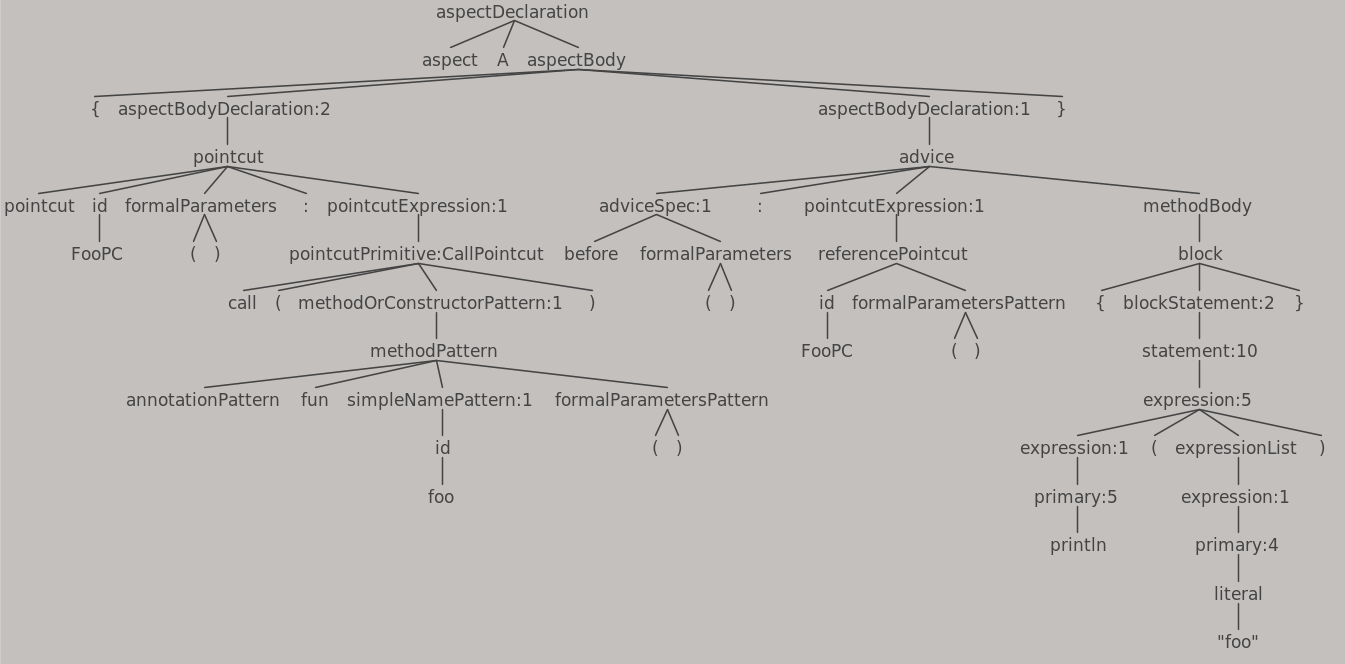
\includegraphics[width=\textwidth]{fig/aspect_parse_plugin.png}
% \caption{Пример разбора аспекта при помощи плагина для ANTRL}%
% \label{fig:aspect_parse_tree}
% \end{figure}

% Как видно из дерева разбора, представленного на рисунке~\ref{fig:aspect_parse_tree}, токены были выделены корректно, а именно:
% \begin{itemize}
%      \item Идентификатор и тело аспекта;
%      \item Идентификатор среза, сигнатура описания среза и описание метода;
%      \item Описание совета и описание среза внутри совета, а также код совета.
% \end{itemize}
% Исходя из анализа этого и ряда других аспектов был сделан вывод о корректности разбора аспекта на токены.

% Следующим этапом проверки корректности разработанного прототипа является проверка корректности построения модели аспекта при помощи функциональных тестов.
% Также на этом этапе, неявно, проверяется корректность сгенерированных по описанной грамматике парсеров и, как следствие, самой грамматики.

% В качестве целевого аспекта возьмем аспект, приведенный в листинге \ref{lst:test_aspect_1}.
% Исходный код теста, предназначенного для проверки корректности построения модели данного аспекта приведен в листинге \ref{lst:test_example_1}:
% \begin{lstlisting}[style={java}, label={lst:test_example_1},
%   caption={Пример теста для проверки корректности построения модели аспекта}]
%     @Test
%     fun visitAspectDeclarationFirst() {
%         val aspect = parseFile("res/aspect_example_1.ak")
%         assertEquals("A", aspect.id)
%         assertEquals(2, aspect.pointcuts.size)

%         val fooPC = aspect.pointcuts.findLast { it.id == "FooPC" }
%         assertNotNull(fooPC)
%         val pointcutExpression = fooPC?.pointcutExpression
%         assertTrue(pointcutExpression is CallNodeItem)
%         assertEquals("foo", (pointcutExpression as CallNodeItem).methodPattern.name.name)
%         assertFalse(pointcutExpression.methodPattern.name.negative)
%         assertEquals(ExtensionType.ANYTHING, pointcutExpression.methodPattern.extensionModifier)
%         assertEquals(InlineType.ANYTHING, pointcutExpression.methodPattern.inlineModifier)

%         val advice = aspect.advices.last()
%         assertTrue(advice is BeforeAdvice)
%         assertEquals("println(\"foo\")",advice.adviceCode.replace("\t", "").replace("\n", "").replace(" ", ""))
%     }
% \end{lstlisting}

% Как видно из листинга~\ref{lst:test_example_1}, в данном тесте проверяется корректность выделения идентификатора аспекта, среза (идентификатора и описания среза) и совета (способ внедрения кода совета, описание среза и код совета).
% При тестировании программы было достигнуто 100\% покрытие тестами классов, отвечающих за построение модели аспектов.

% Следующим этапом проверки качества прототипа является проверка корректности составления срезов и применения советов к точке внедрения.
% Как было сказано ранее, для проведения данной проверки имена вспомогательных методов и переменных генерировались не случайным образом, а были фиксированными.
% При использовании данных ограничений, в ряде случаев на данном этапе невозможна проверка корректности применения множества советов к одной точке объединения, однако, данная проверка будет проводиться на следующем этапе, во время проверки корректности работы программы после применения советов.

% В качестве первого примера рассмотрим применение аспекта, приведенного в листинге~\ref{lst:test_aspect_1}.
% Данный аспект описывает один срез \textit{FooPC}, включающий в себя все места программы, в которых происходит вызов метода \textit{foo()}.
% Совет, содержащийся в аспекте, должен быть применен перед всеми точками объединения, попадающими в срез \textit{FooPC}.
% Код совета содержит в себе вызов метода \textit{println}.
% Рассмотрев целевую программу (приложение~\ref{ch:target_prog}), можно сделать вывод о том, что совет должен быть применен в единственном месте внутри метода \textit{main} --- строке, содержащий код \quotes{f.foo()}.

% В листинге \ref{lst:weaving_example_1} приведено изменение в целевой программе, вызванное применением аспекта.
% \begin{lstlisting}[style={java}, label={lst:weaving_example_1},
%   caption={Пример применения аспекта}]
% f.run{
%     fun adviceFun(){
%         println("foo")
%     }
%     adviceFun()
%     foo()
% }
% \end{lstlisting}

% Как видно из листинга~\ref{lst:weaving_example_1}, преобразования были произведены согласно ожиданиям: точка внедрения была обернута в лямбда-функцию \textit{run}, код совета был помещен внутрь временного метода \textit{adviceFun()}, которая была вызвана до точки внедрения.

% Второй целевой аспект приведен в листинге \ref{lst:aspect_with_target}:
% \begin{lstlisting}[style={java}, label={lst:aspect_with_target},
%   caption={Пример аспекта с сигнатурой \textit{target}}]
% aspect D  {
%     pointcut FooPC(): call(fun foo())

%     after(foo: Foo): target(foo) && FooPC() {
%         foo.baz("Hello baz call")
%     }
% }
% \end{lstlisting}
% Данный аспект имеет срез с идентификатором \textit{FooPC}, аналогичный срезу, представленному в листинге~\ref{lst:test_aspect_1}.
% Описанный в данном срезе совет применяется после точки внедрения и имеет параметр \textit{foo} типа \textit{Foo}, к которому производится обращение внутри кода совета.
% Сигнатура \textit{target(foo)}, говорит о том, что параметр \textit{foo} является элементом, на котором происходит вызов метода, являющегося точкой внедрения.
% Рассмотрев целевую программу (приложение~\ref{ch:target_prog}), можно сделать вывод о том, что совет должен быть применен в единственном месте внутри метода \textit{main} --- строке, содержащий код \quotes{f.foo()}.

% В листинге \ref{lst:weaving_example_2} приведено изменение в целевой программе, вызванное применением аспекта, описанного в листинге \ref{lst:aspect_with_target}.
% \begin{lstlisting}[style={java}, label={lst:weaving_example_2},
%   caption={Пример применения аспекта}]
% f.let{
%     adviceIt ->
%     fun adviceFun(foo: Foo){
%         foo.baz("Hello baz call")
%     }
%     val returnVal = adviceIt.foo()
%     adviceFun(adviceIt)
%     returnVal
% }
% \end{lstlisting}

% Как видно из листинга~\ref{lst:weaving_example_2}, точка внедрения была корректно обернута в лябда-враппер \textit{let}.
% Код совета также был обернут в вспомогательный метод \textit{adviceFun(foo: Foo)}.
% Так как совет содержит параметр, указанный в описании среза в сигнатуре \textit{target}, промежуточный метод принимает первым параметром аргумент такого же типа, что и указанный в сигнатуре \textit{target}.
% При вызове вспомогательного метода внутри враппера в качестве данного параметра передается элемент, на котором происходит вызов целевого метода.
% Ввиду того, что код совета должен быть выполнен после точке внедрения, результат, возвращаемый целевым методом, сохраняется в промежуточной переменной, которая возвращается из враппера.

% По результатам анализа применения набора советов, не было выявлено ошибок, в связи с чем было решено переходить к анализу выполнения программы после применения аспектов.

% Первые эксперименты было решено было проводить на целевой программе, представленной в приложении~\ref{ch:target_prog}.
% Для удобства проверки, на первом этапе было решено использовать вывод отладочных сообщений на консоль.
% Вывод на консоль, получаемый в ходе работы целевой программы представлен в листинге~\ref{lst:output_without_weaving}:
% \begin{lstlisting}[style={java}, label={lst:output_without_weaving},
%   caption={Вывод сообщений в ходе работы целевой программы без применения аспектов}]
% Hello world
% Bar hello
% Say hello again
% Hello from inline
% Bar hello
% PSS Baz!!
% Hello from Bar.bar
% \end{lstlisting}
% Целевая программа организована таким образом, что при вызове метода \textit{foo()} в консоль выводятся строки, соответствующие строкам с 1 по 4 в выводе, представленном в листинге~\ref{lst:output_without_weaving}.

% Текст аспекта, применяемого к программе, приведен в листинге~\ref{lst:around_aspect_example}:
% \begin{lstlisting}[style={java}, label={lst:around_aspect_example},
%   caption={Пример аспекта, используемого для проверки корректности прототипа}]
% aspect E  {
%     pointcut FooPC(): call(fun foo())

%     around(): FooPC() {
%         println("around text")
%     }
% }
% \end{lstlisting}
% Как видно из листинга~\ref{lst:around_aspect_example}, представленный аспект содержит совет \textit{around}, замещающий код точки внедрения кодом совета (в данном случае вызовом метода \quotes{println("around text")}).
% Вывод целевой программы после применения аспектов представлен в листинге~\ref{lst:output_with_weaving}:
% \begin{lstlisting}[style={java}, label={lst:output_with_weaving},
%   caption={Вывод сообщений в ходе работы целевой программы после применения аспекта}]
% around text
% Bar hello
% PSS Baz!!
% Hello from Bar.bar
% \end{lstlisting}

% Как можно судить из вывода, представленного в листинге~\ref{lst:output_with_weaving}, после внедрения аспекта программа работает корректно: она компилируется без ошибок, а также ведет себя после внедрения аспектов согласно ожиданиям (вместо строк, выводимых внутри метода \textit{foo} был вывод, заданный внутри кода совета).

% После того, как работоспособность прототипа была проверена на искусственно созданной программы, было решено проверить работоспособность на реальных проектах. 
% В качестве одной из таких программ было выбрано приложение, вычисляющее значение
% арифметического выражения, заданного в файле.
% В качестве входных данных приложение принимает имя файла, в котором записано
% выражение, а также список значений параметра \textit{x}, используемые при
% вычислении выражения.
% Результатом работы является ассоциативный массив в котором ключем является
% значение параметра, а значением --- результат вычисления выражения при
% подстановке данного значения в качестве значения параметра.

% Программа работает по следующему алгоритму: первым вызывается метод
% \textit{parseExpr}, принимающий имя файла в котором записано выражение и список
% значений параметра.
% Внутри метода \textit{parseExpr} в цикле вызывается метод \textit{calculate}, принимающий
% значение параметра и возвращающий вычисленное значение выражения.
% После чего значение параметра и результат вычисления записывается в
% ассоциативный массив, возвращаемый функцией \textit{parseExpr} в качестве
% результата.
% Также на каждой итерации значение параметра и значения арифметического выражения выводится на консоль.

% Результат работы приложения  без применения аспектов представлен в листинге~\ref{lst:calculate_program_without_weaving}:
% \begin{lstlisting}[style={java}, label={lst:calculate_program_without_weaving},
%   caption={Вывод сообщений в ходе работы целевой программы вычисляющего значения арифметического выражения без применения аспекта}]
% {3=31}
% {31=83590}
% {32=5244871}
% \end{lstlisting}

% Для того, чтобы зафиксировать в журнале время начала и завершения работы метода
% \textit{calculate} воспользуемся аспектом, представленным в листинге
% ~\ref{lst:log_aspect_ex}:
% \begin{lstlisting}[style={java}, label={lst:log_aspect_ex},
%   caption={Пример аспекта, используемого для протоколирования времени начала и конца вызова метода calculate}]
% aspect A  {
%   pointcut pExprPC() : execution(fun parseExpr(String, List<Int>): Map<Int, Int> )
%   pointcut calcPC() : call(fun Expression.calculate(Int): Int)

%   before(): pExprPC() && calcPC() {
%     val l = java.util.logging.Logger.getLogger("ALog")
%     l.info("Start \${System.currentTimeMillis()}")
%   }

%   after(): pExprPC() && calcPC() {
%     val l = java.util.logging.Logger.getLogger("ALog")
%     l.info("Finish \${System.currentTimeMillis()}")
%   }
% }
% \end{lstlisting}
% Как видно из листинга~\ref{lst:log_aspect_ex}, внутри аспекта объявляены два среза: \textit{pExprPC}, включающий в себя все точки внутри тела метода \textit{parseExpr}, и \textit{calcPC}, включающий в себя все места вызова метода \textit{calculate} класса \textit{Expression}.
% Также данный аспект содержит в себе два совета \textit{before} и \textit{after}, выводящие в журнал записи о времени начала и окончания работы метода, являющегося точкой внедрения, соответственно.


% \begin{lstlisting}[style={java}, label={lst:calculate_program_with_weaving},
%   caption={Вывод сообщений в ходе работы целевой программы вычисляющего значения арифметического выражения с применённым аспектом}]
% INFO: Start 1495387830506
% мая 21, 2017 8:30:30 PM MainKt\$parseExpr\$1\$2\$1 invoke
% INFO: Finish 1495387830514
% {3=31}
% мая 21, 2017 8:30:30 PM MainKt\$parseExpr\$1\$1 invoke
% INFO: Start 1495387830522
% мая 21, 2017 8:30:30 PM MainKt\$parseExpr\$1\$2\$1 invoke
% INFO: Finish 1495387830524
% {31=83590}
% мая 21, 2017 8:30:30 PM MainKt\$parseExpr\$1\$1 invoke
% INFO: Start 1495387830528
% мая 21, 2017 8:30:30 PM MainKt\$parseExpr\$1\$2\$1 invoke
% INFO: Finish 1495387830534
% {32=5244871}
% \end{lstlisting}

%%%%%%%%%%%%%%%%%%%%%%%%%%%%%%%%%%%%%%%%%%%%%%%%%%%%%%%%%%%%%%%%%%%%%%%%%%%%%%%%
\section{Выводы}
\label{sec:ch5_conclusion}
%%%%%%%%%%%%%%%%%%%%%%%%%%%%%%%%%%%%%%%%%%%%%%%%%%%%%%%%%%%%%%%%%%%%%%%%%%%%%%%%
Тестирование разработанного прототипа показало его соответствие сформулированным требованиям:
\begin{itemize}
	\item Возможность применения советов до, после и вместо точки внедрения.
	\item Возможность использования сигнатур \textit{call}, \textit{execution} и \textit{target} при описании срезов.
	\item Возможность использования логических операций \quotes{и} \quotes{или} \quotes{не}.
\end{itemize}
В ходе проверки корректности работы прототипа не было обнаружено ошибок.
%%%%%%%%%%%%%%%%%%%%%%%%%%%%%%%%%%%%%%%%%%%%%%%%%%%%%%%%%%%%%%%%%%%%%%%%%%%%%%%%
